\begin{frame}%
    \frametitle{Feature branches}%
    \monocolumn{
	    \only<1>{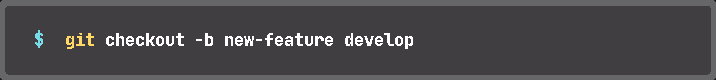
\includegraphics{img/code/start-new-feature.pdf}}%
	    \only<2>{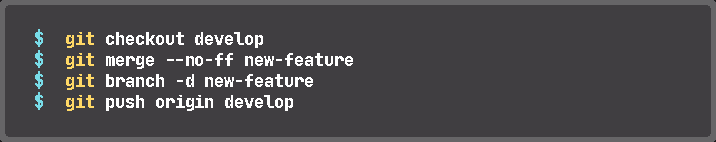
\includegraphics{img/code/finish-new-feature.pdf}}%
	}
%
    \only<3>{\monocolumn{\resizebox{.6\paperwidth}{!}{
    	\begin{tikzpicture}
	    	\node[rotate=90] (git-graph-upper) {%
	   			\begin{tikzpicture}[%
	   				git graph,
	   				remember picture,
   				]
	   				\matrix[%
		   				column sep=-.5em,
		   				row sep=.5em,
		   				column 1/.style = {nodes={%
	   						style=feature,
	   						xshift=-1.35\columnsep,
		   				}},
		   				column 2/.style = {nodes={%
	   						style=develop,
	   						xshift=-1.35\columnsep,
		   				}},
		   				ampersand replacement=\&
	  				] (git-graph-matrix) {%
	   					\ghost{feature}     \& \ghost{develop}     \\
	   					                    \& \commit{develop-01} \\
	   					                    \& \commit{develop-02} \\
	   					\commit{feature-03} \&                     \\
	   					\commit{feature-04} \&                     \\
	   					\commit{feature-05} \&                     \\
	   					                    \& \commit{develop-06} \\
	   				};
   				%
   					\foreach \branch/\branchcolour in {%
   						develop/monokai-yellow,
   						feature/monokai-orange%
   					}{%
						\node[%
	 						anchor = east,
	 						inner sep = 2pt,
	 						baseline = (subsection-text.base),
	 						font = \fontsize{4}{5}\selectfont,
	 						rotate = -90,
	 						xshift = -.5em,
						] (branch-label) at (\branch.west) {%
							\fontfamily{JetBrainsMono-SemiBold}\selectfont%
							\defaultfontfeatures{LetterSpace=10}%
							\ttfamily\bfseries\color{monokai-bg}%
							\strut\branch
						};
					%
 						\begin{pgfonlayer}{background}%
 							\fill[%
	  							\branchcolour,
	  							rounded corners = 1pt,
 							]%
	  							([shift={(-1.75pt,0pt)}]branch-label.north west)%
	  							rectangle%
	  							([shift={(2.25pt,0pt)}]branch-label.south east);%
 						%
 							\draw[%
	 							monokai-grey-400,
	 							ultra thin,
 							]%
	 							(\branch)%
	 							--%
	 							([yshift=-1em]\branch|-develop-06) node [] {};
 						\end{pgfonlayer}%
   					}
 				%
   					\begin{pgfonlayer}{background}%
	   					\foreach \fromcommit/\tocommit in {%
	   						develop-01/develop-02,
	   						develop-02/feature-03,
	   						feature-03/feature-04,
	   						feature-04/feature-05,
	   						feature-05/develop-06%
	   					}{
	   						\connect{\fromcommit}{\tocommit};
	   					}
	   				\end{pgfonlayer}%
   				%
   					\draw[%
	   					decorate,
	   					decoration={%
	   						brace,
	   						amplitude=3pt,
	   						mirror,
	   						raise=4pt,
	   					},
	   					yshift=0pt,
   					]%
	   					(feature-03.north west)%
	   					--%
	   					(feature-05.south west)%
	   					node [
	   						text = monokai-orange,
	   						midway,
	   						rotate = -90,
	   						font = \fontsize{4}{5}\selectfont,
	   						yshift=-6pt,
	   						anchor=north,
	   					] {\tiny\itshape feature};
	   			\end{tikzpicture}%
	   		};
   		%
   			\draw[%
   				monokai-grey-100,
   				->,
   				>=stealth,
   			]%
	   			([shift={(10.75mm,-2.5mm)}]git-graph-upper.north east)%
	   			--%
	   			([shift={(-2.5mm,-2.5mm)}]git-graph-upper.south east)%
	   			node[midway, above] {\tiny Time};
	   	%
	   	%
	   	%
	   		\node[rotate=90] (git-graph-lower) at ([shift={(-.13em,-.5em)}]git-graph-upper.west) {%
	   			\begin{tikzpicture}[%
	   				git graph,
	   				remember picture,
   				]
	   				\matrix[%
		   				column sep=-.5em,
		   				row sep=.5em,
		   				column 1/.style = {nodes={%
		   						style=feature,
		   						xshift=-1.35\columnsep,
		   				}},
		   				column 2/.style = {nodes={%
		   						style=develop,
		   						xshift=-1.35\columnsep,
		   				}},
		   				ampersand replacement=\&
	   				] (git-graph-matrix) {%
	   					\ghost{feature} \& \ghost{develop}      \\
	   					                \& \commit{develop-01}  \\
	   					                \& \commit{develop-02}  \\
	   					                \& \commit{develop-03}  \\
	   					                \& \commit{develop-04}  \\
	   					                \& \commit{develop-05}  \\
	   					                \& \ghost{develop-null} \\
	   				};
   				%
	   				\foreach \branch/\branchcolour in {%
	   					develop/monokai-yellow,
	   					feature/monokai-orange%
	   				}{%
	   					\node[%
		   					anchor = east,
		   					inner sep = 2pt,
		   					baseline = (subsection-text.base),
		   					font = \fontsize{4}{5}\selectfont,
		   					rotate = -90,
		   					xshift = -.5em,
	   					] (branch-label) at (\branch.west) {%
	   						\fontfamily{JetBrainsMono-SemiBold}\selectfont%
	   						\defaultfontfeatures{LetterSpace=10}%
	   						\ttfamily\bfseries\color{monokai-bg}%
	   						\strut\branch
	   					};
   					%
	   					\begin{pgfonlayer}{background}%
	   						\fill[%
		   						\branchcolour,
		   						rounded corners = 1pt,
	   						]%
		   						([shift={(-1.75pt,0pt)}]branch-label.north west)%
		   						rectangle%
		   						([shift={(2.25pt,0pt)}]branch-label.south east);%
   						%
	   						\draw[%
		   						monokai-grey-400,
		   						ultra thin,
	   						]%
		   						(\branch)%
		   						--%
		   						([yshift=-1em]\branch|-develop-06) node [] {};
	   					\end{pgfonlayer}%
	   				}
   				%
	   				\begin{pgfonlayer}{background}%
	   					\foreach \fromcommit/\tocommit in {%
	   						develop-01/develop-02,
	   						develop-02/develop-03,
	   						develop-03/develop-04,
	   						develop-04/develop-05%
	   					}{
	   						\connect{\fromcommit}{\tocommit};
	   					}
	   				\end{pgfonlayer}%
   				%
	   				\draw[%
		   				decorate,
		   				decoration={%
		   					brace,
		   					amplitude=3pt,
%			   				mirror,
		   					raise=4pt,
		   				},
		   				yshift=0pt,
	   				]%
		   				(develop-03.north east)%
		   				--%
		   				(develop-05.south east);
		   		%
		   			\draw[
		   				monokai-accent-colour,
		   				dash pattern=on 1.5pt off .5pt,
		   				thick,
		   				rounded corners = 1pt,
		   			]
		   				([shift={(2pt,2pt)}]develop-03.north east)%
		   				-- ++(-1.5em, 0em)%
		   				-- ++(0em, -2.5em-1.5pt)%
		   				-- ++(1.5em, 0em)%
		   				-- cycle;
	   			\end{tikzpicture}%
	   		};
   		%
   			\node[%
	   			anchor = east,
	   			inner sep = 2pt,
	   			baseline = (subsection-text.base),
	   			font = \fontsize{4}{5}\selectfont,
%	   			xshift = -.5em,
   			] (branch-label) at (git-graph-upper.north) {%
   				\ttfamily\bfseries\color{monokai-fg}%
   				\strut\textcolor{monokai-yellow}{git} merge --no-ff%
   			};
   		%
   			\node[%
	   			anchor = east,
	   			inner sep = 2pt,
	   			baseline = (subsection-text.base),
	   			font = \fontsize{4}{5}\selectfont,
%	   			xshift = -.5em,
   			] (branch-label) at ([yshift=-.6em]git-graph-lower.north) {%
   				\ttfamily\bfseries\color{monokai-fg}%
   				\strut\textcolor{monokai-yellow}{git} merge%
   			};
   		\end{tikzpicture}
	}}}
\end{frame}%